%% ========================================================================
%% Latex Template for CSC4006: Research and Development Project
%% Adapted in September 2018 by Dr Blesson Varghese from the IEEE Template
%% School of Electronics, Electrical Engineering and Computer Science
%% Queen's University Belfast, UK
%% ========================================================================


\documentclass[journal]{IEEEtran}
%
% If IEEEtran.cls has not been installed into the LaTeX system files,
% manually specify the path to it like:
% \documentclass[journal]{../sty/IEEEtran}


% Some very useful LaTeX packages include:
% (uncomment the ones you want to load)


% *** MISC UTILITY PACKAGES ***
%
%\usepackage{ifpdf}
% Heiko Oberdiek's ifpdf.sty is very useful if you need conditional
% compilation based on whether the output is pdf or dvi.
% usage:
% \ifpdf
%   % pdf code
% \else
%   % dvi code
% \fi
% The latest version of ifpdf.sty can be obtained from:
% http://www.ctan.org/pkg/ifpdf
% Also, note that IEEEtran.cls V1.7 and later provides a builtin
% \ifCLASSINFOpdf conditional that works the same way.
% When switching from latex to pdflatex and vice-versa, the compiler may
% have to be run twice to clear warning/error messages.





\usepackage{hyperref}

% *** CITATION PACKAGES ***
%
\usepackage{cite}
% cite.sty was written by Donald Arseneau
% V1.6 and later of IEEEtran pre-defines the format of the cite.sty package
% \cite{} output to follow that of the IEEE. Loading the cite package will
% result in citation numbers being automatically sorted and properly
% "compressed/ranged". e.g., [1], [9], [2], [7], [5], [6] without using
% cite.sty will become [1], [2], [5]--[7], [9] using cite.sty. cite.sty's
% \cite will automatically add leading space, if needed. Use cite.sty's
% noadjust option (cite.sty V3.8 and later) if you want to turn this off
% such as if a citation ever needs to be enclosed in parenthesis.
% cite.sty is already installed on most LaTeX systems. Be sure and use
% version 5.0 (2009-03-20) and later if using hyperref.sty.
% The latest version can be obtained at:
% http://www.ctan.org/pkg/cite
% The documentation is contained in the cite.sty file itself.






% *** GRAPHICS RELATED PACKAGES ***
%
\ifCLASSINFOpdf
  \usepackage[pdftex]{graphicx}
  \usepackage{extramarks}
  % declare the path(s) where your graphic files are
  % \graphicspath{{../pdf/}{../jpeg/}}
  % and their extensions so you won't have to specify these with
  % every instance of \includegraphics
  % \DeclareGraphicsExtensions{.pdf,.jpeg,.png}
\else
  % or other class option (dvipsone, dvipdf, if not using dvips). graphicx
  % will default to the driver specified in the system graphics.cfg if no
  % driver is specified.
  % \usepackage[dvips]{graphicx}
  % declare the path(s) where your graphic files are
  % \graphicspath{{../eps/}}
  % and their extensions so you won't have to specify these with
  % every instance of \includegraphics
  % \DeclareGraphicsExtensions{.eps}
\fi
% graphicx was written by David Carlisle and Sebastian Rahtz. It is
% required if you want graphics, photos, etc. graphicx.sty is already
% installed on most LaTeX systems. The latest version and documentation
% can be obtained at: 
% http://www.ctan.org/pkg/graphicx
% Another good source of documentation is "Using Imported Graphics in
% LaTeX2e" by Keith Reckdahl which can be found at:
% http://www.ctan.org/pkg/epslatex
%
% latex, and pdflatex in dvi mode, support graphics in encapsulated
% postscript (.eps) format. pdflatex in pdf mode supports graphics
% in .pdf, .jpeg, .png and .mps (metapost) formats. Users should ensure
% that all non-photo figures use a vector format (.eps, .pdf, .mps) and
% not a bitmapped formats (.jpeg, .png). The IEEE frowns on bitmapped formats
% which can result in "jaggedy"/blurry rendering of lines and letters as
% well as large increases in file sizes.
%
% You can find documentation about the pdfTeX application at:
% http://www.tug.org/applications/pdftex





% *** MATH PACKAGES ***
%
%\usepackage{amsmath}
% A popular package from the American Mathematical Society that provides
% many useful and powerful commands for dealing with mathematics.
%
% Note that the amsmath package sets \interdisplaylinepenalty to 10000
% thus preventing page breaks from occurring within multiline equations. Use:
%\interdisplaylinepenalty=2500
% after loading amsmath to restore such page breaks as IEEEtran.cls normally
% does. amsmath.sty is already installed on most LaTeX systems. The latest
% version and documentation can be obtained at:
% http://www.ctan.org/pkg/amsmath





% *** SPECIALIZED LIST PACKAGES ***
%
%\usepackage{algorithmic}
% algorithmic.sty was written by Peter Williams and Rogerio Brito.
% This package provides an algorithmic environment fo describing algorithms.
% You can use the algorithmic environment in-text or within a figure
% environment to provide for a floating algorithm. Do NOT use the algorithm
% floating environment provided by algorithm.sty (by the same authors) or
% algorithm2e.sty (by Christophe Fiorio) as the IEEE does not use dedicated
% algorithm float types and packages that provide these will not provide
% correct IEEE style captions. The latest version and documentation of
% algorithmic.sty can be obtained at:
% http://www.ctan.org/pkg/algorithms
% Also of interest may be the (relatively newer and more customizable)
% algorithmicx.sty package by Szasz Janos:
% http://www.ctan.org/pkg/algorithmicx




% *** ALIGNMENT PACKAGES ***
%
%\usepackage{array}
% Frank Mittelbach's and David Carlisle's array.sty patches and improves
% the standard LaTeX2e array and tabular environments to provide better
% appearance and additional user controls. As the default LaTeX2e table
% generation code is lacking to the point of almost being broken with
% respect to the quality of the end results, all users are strongly
% advised to use an enhanced (at the very least that provided by array.sty)
% set of table tools. array.sty is already installed on most systems. The
% latest version and documentation can be obtained at:
% http://www.ctan.org/pkg/array


% IEEEtran contains the IEEEeqnarray family of commands that can be used to
% generate multiline equations as well as matrices, tables, etc., of high
% quality.




% *** SUBFIGURE PACKAGES ***
%\ifCLASSOPTIONcompsoc
%  \usepackage[caption=false,font=normalsize,labelfont=sf,textfont=sf]{subfig}
%\else
%  \usepackage[caption=false,font=footnotesize]{subfig}
%\fi
% subfig.sty, written by Steven Douglas Cochran, is the modern replacement
% for subfigure.sty, the latter of which is no longer maintained and is
% incompatible with some LaTeX packages including fixltx2e. However,
% subfig.sty requires and automatically loads Axel Sommerfeldt's caption.sty
% which will override IEEEtran.cls' handling of captions and this will result
% in non-IEEE style figure/table captions. To prevent this problem, be sure
% and invoke subfig.sty's "caption=false" package option (available since
% subfig.sty version 1.3, 2005/06/28) as this is will preserve IEEEtran.cls
% handling of captions.
% Note that the Computer Society format requires a larger sans serif font
% than the serif footnote size font used in traditional IEEE formatting
% and thus the need to invoke different subfig.sty package options depending
% on whether compsoc mode has been enabled.
%
% The latest version and documentation of subfig.sty can be obtained at:
% http://www.ctan.org/pkg/subfig




% *** FLOAT PACKAGES ***
%
%\usepackage{fixltx2e}
% fixltx2e, the successor to the earlier fix2col.sty, was written by
% Frank Mittelbach and David Carlisle. This package corrects a few problems
% in the LaTeX2e kernel, the most notable of which is that in current
% LaTeX2e releases, the ordering of single and double column floats is not
% guaranteed to be preserved. Thus, an unpatched LaTeX2e can allow a
% single column figure to be placed prior to an earlier double column
% figure.
% Be aware that LaTeX2e kernels dated 2015 and later have fixltx2e.sty's
% corrections already built into the system in which case a warning will
% be issued if an attempt is made to load fixltx2e.sty as it is no longer
% needed.
% The latest version and documentation can be found at:
% http://www.ctan.org/pkg/fixltx2e


%\usepackage{stfloats}
% stfloats.sty was written by Sigitas Tolusis. This package gives LaTeX2e
% the ability to do double column floats at the bottom of the page as well
% as the top. (e.g., "\begin{figure*}[!b]" is not normally possible in
% LaTeX2e). It also provides a command:
%\fnbelowfloat
% to enable the placement of footnotes below bottom floats (the standard
% LaTeX2e kernel puts them above bottom floats). This is an invasive package
% which rewrites many portions of the LaTeX2e float routines. It may not work
% with other packages that modify the LaTeX2e float routines. The latest
% version and documentation can be obtained at:
% http://www.ctan.org/pkg/stfloats
% Do not use the stfloats baselinefloat ability as the IEEE does not allow
% \baselineskip to stretch. Authors submitting work to the IEEE should note
% that the IEEE rarely uses double column equations and that authors should try
% to avoid such use. Do not be tempted to use the cuted.sty or midfloat.sty
% packages (also by Sigitas Tolusis) as the IEEE does not format its papers in
% such ways.
% Do not attempt to use stfloats with fixltx2e as they are incompatible.
% Instead, use Morten Hogholm'a dblfloatfix which combines the features
% of both fixltx2e and stfloats:
%
% \usepackage{dblfloatfix}
% The latest version can be found at:
% http://www.ctan.org/pkg/dblfloatfix




%\ifCLASSOPTIONcaptionsoff
%  \usepackage[nomarkers]{endfloat}
% \let\MYoriglatexcaption\caption
% \renewcommand{\caption}[2][\relax]{\MYoriglatexcaption[#2]{#2}}
%\fi
% endfloat.sty was written by James Darrell McCauley, Jeff Goldberg and 
% Axel Sommerfeldt. This package may be useful when used in conjunction with 
% IEEEtran.cls'  captionsoff option. Some IEEE journals/societies require that
% submissions have lists of figures/tables at the end of the paper and that
% figures/tables without any captions are placed on a page by themselves at
% the end of the document. If needed, the draftcls IEEEtran class option or
% \CLASSINPUTbaselinestretch interface can be used to increase the line
% spacing as well. Be sure and use the nomarkers option of endfloat to
% prevent endfloat from "marking" where the figures would have been placed
% in the text. The two hack lines of code above are a slight modification of
% that suggested by in the endfloat docs (section 8.4.1) to ensure that
% the full captions always appear in the list of figures/tables - even if
% the user used the short optional argument of \caption[]{}.
% IEEE papers do not typically make use of \caption[]'s optional argument,
% so this should not be an issue. A similar trick can be used to disable
% captions of packages such as subfig.sty that lack options to turn off
% the subcaptions:
% For subfig.sty:
% \let\MYorigsubfloat\subfloat
% \renewcommand{\subfloat}[2][\relax]{\MYorigsubfloat[]{#2}}
% However, the above trick will not work if both optional arguments of
% the \subfloat command are used. Furthermore, there needs to be a
% description of each subfigure *somewhere* and endfloat does not add
% subfigure captions to its list of figures. Thus, the best approach is to
% avoid the use of subfigure captions (many IEEE journals avoid them anyway)
% and instead reference/explain all the subfigures within the main caption.
% The latest version of endfloat.sty and its documentation can obtained at:
% http://www.ctan.org/pkg/endfloat
%
% The IEEEtran \ifCLASSOPTIONcaptionsoff conditional can also be used
% later in the document, say, to conditionally put the References on a 
% page by themselves.




% *** PDF, URL AND HYPERLINK PACKAGES ***
%
%\usepackage{url}
% url.sty was written by Donald Arseneau. It provides better support for
% handling and breaking URLs. url.sty is already installed on most LaTeX
% systems. The latest version and documentation can be obtained at:
% http://www.ctan.org/pkg/url
% Basically, \url{my_url_here}.




% *** Do not adjust lengths that control margins, column widths, etc. ***
% *** Do not use packages that alter fonts (such as pslatex).         ***
% There should be no need to do such things with IEEEtran.cls V1.6 and later.
% (Unless specifically asked to do so by the journal or conference you plan
% to submit to, of course. )


% correct bad hyphenation here
\hyphenation{op-tical net-works semi-conduc-tor}


\begin{document}

% Titles are generally capitalized except for words such as a, an, and, as,
% at, but, by, for, in, nor, of, on, or, the, to and up, which are usually
% not capitalized unless they are the first or last word of the title.
% Linebreaks \\ can be used within to get better formatting as desired.
% Do not put math or special symbols in the title.
\title{GitSlice: Slicing the Repository That Feeds Us}

% author names and IEEE memberships
% note positions of commas and nonbreaking spaces ( ~ ) LaTeX will not break
% a structure at a ~ so this keeps an author's name from being broken across
% two lines.
% use \thanks{} to gain access to the first footnote area
% a separate \thanks must be used for each paragraph as LaTeX2e's \thanks
% was not built to handle multiple paragraphs
%
\author{Dylan Wilson \textless\texttt{dwilson402@qub.ac.uk}\textgreater \\ Queen's University Belfast }

\markboth{CSC4006: Research and Development Project}{}%

%If there are multiple Authors
% {Varghese \MakeLowercase{\textit{et al.}}: Template for Research Article}
% The only time the second header will appear is for the odd numbered pages
% after the title page when using the twoside option.
% 
% *** Note that you probably will NOT want to include the author's ***
% *** name in the headers of peer review papers.                   ***
% You can use \ifCLASSOPTIONpeerreview for conditional compilation here if
% you desire.


% make the title area
\maketitle

% As a general rule, do not put math, special symbols or citations
% in the abstract or keywords.
\begin{abstract}
Professional software development teams now almost universally use Git (a distributed version control system) to manage changes to their code.
Git repositories contain metadata relating to the development of the project and show how a project has changed over time.
Analysis of this metadata to gain insight into the software development process is performed in the field of mining software repositories (MSR).
Static code analysis (SCA) tools perform analysis on source code to detect issues during development (they are static because they analyse the code without running it) such as untested or vulnerable code.
SCA only analyses one version of the code, however.
The ability to run code analysis tools across many versions of a project could therefore provide developers with useful information of how their code changes over time.
To achieve this, a tool, GitSlice will be built to iterate through a given set of Git commits to run a code analysis tool on each version of the software and provide the developer with information about how metrics of their code change over time.
Iterating through commits in a linear fashion is slow, so to reduce the time taken to iterate through the commits we will parallelize this process.

\end{abstract}

\begin{IEEEkeywords}
Version control systems, Mining software repositories, High-performance computing.
\end{IEEEkeywords}

\IEEEpeerreviewmaketitle

\section{Introduction}
\label{sec:introduction}
Today, virtually all professional and open-source development teams use version control systems (VCSs) to manage changes in their projects.
StackOverflow reports over 96\% of professional developers use Git~\cite{vcs_usage}.
Git is a distributed VCS developed originally by Linus Torvalds and other contributors to the Linux kernel.
Version control systems enable developers to manage changes to code in their software projects.
A set of changes in Git is known as a commit~\cite{pro_git}.
Each commit points to one or more previous commits to form a tree (except for the first commit known as the root commit).
Multiple commits can have the same parent, which allows for a branching model and commits which have multiple parents merge two or more branches together.
\autoref{fig:git_branching} shows the Git branching model visually.

\begin{figure}[ht]
	\centering
	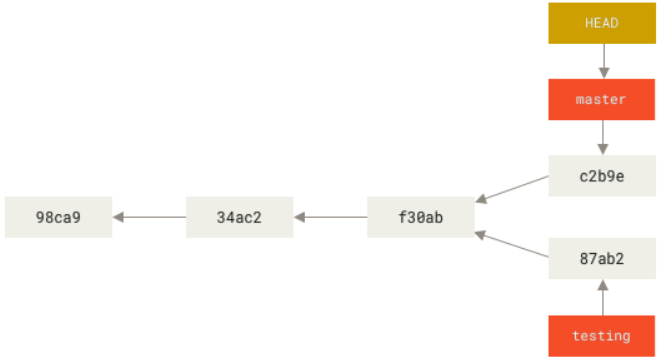
\includegraphics[width=0.35\textwidth]{images/git-branching}
	\caption{Git branching model, two branches exist one called master and one called testing~\cite{pro_git}.}
\label{fig:git_branching}
\end{figure}

Commits contain more information than just changes to file contents - they also include information about who authored the commit and who last applied it (for example, when a commit is imported from a patch file or when the commit is part of a rebase)---known as the author and committer respectively.
The field of mining software repositories (MSR) attempts to analyze the contents of software repositories to obtain useful information about a software project~\cite{road_ahead_for_msr}.

Code analysis tools are used to understand the quality of software code such as test coverage and security vulnerabilities.
Tools which do not run the code but instead analyse the code by reading it are called static code analysis.
One common type of static code analysis is static application security testing (SAST).
A SAST tool such a Snyk Code or SonarQube Security Analysis will analyze the code to detect common security vulnerabilities such as the use of known weak hashing or encryption algorithms, or known vulnerable dependency versions~\cite{scat}.
One common limitation of these tools, however, is that they only perform analysis on one version of the software.
It is possible then that an older version of the project used a dependency which has since had a vulnerability discovered---if the vulnerability is not present in a later version of the dependency (a version which the current version of the software project uses) then the SAST tool will not identify this vulnerability.
Similarly, as these tools continually improve and can detect more types of vulnerability it is possible that an older version of the project contains a vulnerability which was not initially discovered but running the tool again would result in it detecting the vulnerability.
This older version of the software could still be deployed, however and so identifying vulnerabilities in older versions of software is still important.

Another example of static code analysis is code coverage of software testing.
This type of tool will run tests written for the software and calculate the percentage of the program tested and which lines are untested.
While it could be useful for software development teams to see the trend in code coverage over time, code coverage tools typically only perform code coverage on the current version of the code.

A tool which performs analysis on multiple versions of the project could show a time-series graph to show how metrics change over time.
One example of this a graph which shows how the percentage of code covered by tests changes over time.

Iterating through each version of the project sequentially and running analysis is slow (the Linux repository for example has over 1.3m commits as of Dec 2022 and if each commit only took 1 second to be checked out and built it would still take 15 days to go through every commit~\cite{linux_git}).
Each version of the program does not depend on other versions previously having been built so parallelization can be used to significantly speed up this process.
Each process could use an isolated environment to avoid overwriting output from other processes.



\section{Literature Review}
\label{sec:literature-review}
\textbf{Mining software repositories:} The mining software repositories (MSR) field analyses software repositories to find actionable information about software projects~\cite{msrconf}.
In MSR studies, researchers extract data from a repository to produce evidence to answer a research question~\cite{road_ahead_for_msr}.
While software repositories are typically used as historical records of the software development process, MSR attempts to use the information contained within them to guide future decisions.

Many tools exist to analyse software evolution but these primarily focus on metadata.
For example, one such tool is Boa~\cite{boa} which uses a domain-specific language (DSL) to describe how to mine a selection of software repositories from SourceForge and GitHub.
This enables researchers to write DSL for questions like ``How many files are changed on average per commit in projects which use Java?''.
The tool will then iterate through each commit in every Java project on SourceForge and GitHub to produce the answer.
Boa, however, does not allow for the running of a specific tool on each iteration but rather simply extracting metadata from the commits of the repository.

Similarly to Boa,~\cite{closer} introduces CLOSER which is a DSL for metadata across multiple types of VCS'.
This allows for the conversion of a software repository from one type of VCS to another.
CLOSER primarily focuses on the metadata of a repository (as opposed to each version of code stored within in it) but has provided a starting point for research into this area.

Another is example is described in \cite{libvcs4j} which introduces LibVCS4j, a Java library which enables the mining of software repositories.
LibVCS4j supports multiple types of repository and abstracts the specific VCS away at an API level to enable the mining of data from multiple types of repositories.
Again, however, this library primarily focuses on enabling the mining of metadata from the repository as opposed to performing analysis on the code itself.

\cite{cvsgrab} describes CVSgrab is a tool for visualizing metadata of a CVS repository (an older VCS than Git).
This allows for visualization of different metadata such as the types of files and authors of lines of code.
The tool produces a graph which shows how this metadata changes over time.
CVSgrab however, is built for CVS and doesn't allow the running of any tool on each version of the software but merely one type of visualization of the data contained within the repository.

\cite{mjgit} describes MJgit, a tool which performs code analysis on changes to code in a project by understanding how these changes affect the code.
This allows for better textual search of the source code by ignoring cases where methods were simply moved but their functionality did not change (this would be registered in Git as line deletions then line additions, but wouldn't be included in the search results for MJgit) allowing for more accurate searching of the repository.

\textbf{Source code analytics:}~\cite{sonarqube} compared the features of the three most commonly presented tools for static code analysis in research: Cppcheck, FindBugs and SonarQube.
The finding was of all the features compared, SonarQube provided the greatest feature set.
SonarQube also supports more languages than the other two where Cppcheck only supports C/C++ and FindBugs only supports Java.
Therefore, SonarQube could be used to perform static code analysis on many types of project, and therefore a good potential candidate for a tool to validate any approach.

\cite{java_ci_sca} investigates the use of static code analysis in the CI/CD pipelines of 20 open-source Java projects.
A majority of projects used tool called CheckStyle which checks adherence to a set of rules on code style.
CheckStyle is another tool which could be used to validate the approach by understanding how rule violations vary over time.
Further, the use of GitSlice in the CI/CD pipeline would enable developers to continually run their static code analysis tools on previous versions of the project.
For example, running GitSlice upon push to a mainline or release branch would ensure older versions are continually checked.

\cite{li_2020} analysed the benefits and limitations of Checkmarx, a common static application security testing (SAST).
This is another good example of a tool which could be used to validate the approach by creating known vulnerable code between specific commits and testing to see if the tool is able to use Checkmarx to find the vulnerability.

\textbf{Running at scale:}~\cite{torcpy} describes torcpy, a load-balancing Python library which manages the execution of multiple asynchronous tasks and supports OpenMPI which is an open-source MPI implementation that is widely used on computing clusters including Perlmutter, the 8th most powerful supercomputer according to the Nov 2022 TOP500 rankings~\cite{perlmutter}.
This enables multiple versions of the program to run across nodes in a cluster, balancing workload to ensure optimal use of resources.

Some existing work has been done in relation to accessing Git repositories in high-performance computing environments such as RepoFS~\cite{repofs}, a tool for accessing multiple versions of the repository.
RepoFS exposes the commits of the repository as a virtual filesystem, ordered in a tree structure by metadata from the commit by both commit ID and by date of the commit.
Use of RepoFS would allow a highly parallelised analysis to be performed on a shared filesystem against a single copy of a repository rather than making multiple copies each at a specific point.

Running multiple versions of the same program can lead to issues, for example SonarQube will fail to run if another instance is already scanning the same project~\cite{sonarqube_parallel}.
Containers, such as Docker, enable the isolation of a process from the rest of the operating system and ensures that the process will run predictably across different platforms~\cite{container_benefits}.
Running the code analysis tool inside a container also means it will be isolated (including its filesystem) from the other processes on the system allowing for multiple versions of the same tool to run simultaneously without interacting with each other.
An analysis of Docker in high-performance environments shows that this also provides performance similar to that of running the software natively (i.e.\ directly on the operating system without any visualisation) and much greater than that of running it inside virtual machines~\cite{docker_hpc}.


\newpage

\appendix[Current work]
To date an application written in Python has been partially developed~\cite{gitlab}.
The application uses the GitPython package to interact with the Git repository.
The program reads from a configuration file (written in YAML) at the location passed as an argument.
This file contains options such as the repository to be analysed, the Docker image containing the analysis tools to be used, and the command to run to start the container.
It will then copy a local Git repository (later, it will be able to clone a remote repository) and copy it into a working directory.
The application gets each commit in the repository and will checkout that version in an incremental fashion.
For each commit, the Docker image specified by the configuration file will be pulled and a container based on this image run.
The project (as it existed at the commit to be analysed) will be mounted on the container and the command provided in the configuration file will be run to begin the analysis.
When the container exits, it's output (both stdin and stderr) is output to the screen.
This represents a basic, working version of what we aim to develop.

There are some limitations with this current version -- the most obvious of which is that every commit in the repository is checked-out and run, later the configuration file will be read to identify which set of commits should be checked-out for example, every 5th commit from the year 2019.
Further, the output of the container is simply printed to the screen and not useful work is done to interpret this.
As previously mentioned, the ability to clone the repository directly from a remote will also be added.
Later versions of the application could save the output of each run to a directory to allow further analysis to be performed on the output, some additional features to interpret the output and display graphs could also be added (for example, by grepping for a particular value in the output).
The application currently runs each commit in a sequential fashion so changes will be made to parallelize the code so that multiple versions of the repository can be checked out and run in parallel.
The packages mentioned in the previous section will be used to achieve this.
To use the RepoFS tool on Kelvin 2 it is necessary to build the libgit2 headers from source (we cannot install packages here) -- this will be handled by the program upon starting up on each node.
It is possible to use run containers on Kelvin 2 using the Singularity module, further work will be done into how to extract a container as an .iso file and run this in singularity programmatically.

% Can use something like this to put references on a page
% by themselves when using endfloat and the captionsoff option.
\ifCLASSOPTIONcaptionsoff
  \newpage
\fi



% trigger a \newpage just before the given reference
% number - used to balance the columns on the last page
% adjust value as needed - may need to be readjusted if
% the document is modified later
%\IEEEtriggeratref{8}
% The "triggered" command can be changed if desired:
%\IEEEtriggercmd{\enlargethispage{-5in}}

% references section

% can use a bibliography generated by BibTeX as a .bbl file
% BibTeX documentation can be easily obtained at:
% http://mirror.ctan.org/biblio/bibtex/contrib/doc/
% The IEEEtran BibTeX style support page is at:
% http://www.michaelshell.org/tex/ieeetran/bibtex/
%\bibliographystyle{IEEEtran}
% argument is your BibTeX string definitions and bibliography database(s)
%\bibliography{IEEEabrv,../bib/paper}
%
% <OR> manually copy in the resultant .bbl file
% set second argument of \begin to the number of references
% (used to reserve space for the reference number labels box)
\bibliographystyle{IEEEtran}  
\bibliography{references}


% that's all folks
\end{document}


